\chapter{Muestra y técnicas experimentales}
\label{chap:techniques-and-sample}
\textit{En este capítulo discutiremos los principales aspectos de la muestra estudiada y las técnicas utilizadas para la 
caracterización de la misma.}
\vfill
\minitoc
\newpage

\section{Descripción de las muestras.}
\label{sec:chap3-sample-description}
Las muestras estudiadas son los cristales de CdTe (001) y Hg$_{0.18}$Cd$_{0.82}$Te (001). En el caso del CdTe es una muestra no dopada intencionalmente ($ 5.6\times10^{16}\ cm^{-3} $). En el caso del cristal de Hg$_{0.18}$Cd$_{0.82}$T (001), este consiste de una capa de Hg$_{0.18}$Cd$_{0.82}$Te (001) de $ 1\ \mu m $ de espesor crecida sobre un sustrato de CdTe (001). Las propiedades ópticas de ambos cristales han sido detalladamente estudiadas en los laboratorios del IICO por medio de Elipsometria Espectroscópica \cite{Camacho2005, LastrasMartnez2009}. El análisis y obtención de los parámetros ópticos han sido realizados tanto en el espacio directo como en el espacio inverso\cite{Camacho2005, LastrasMartnez2009}.

En la Tabla \ref{tab:crystal_description}, se condensa la información de los cristales estudiados, contra el prístino con el que se compararon sus propiedades y las técnicas utilizadas para su caracterización.

\begin{table}[h!]
    \centering
        \begin{tabular}{m{7em} m{5em} m{8em} m{12em}}
        \hline \hline
        Cristal 		            & Orientación   & Condición         & Técnicas utilizadas\\
        \hline
        CdTe                        & (001)         & Deposición de Ag 	& AFM-NSOM, Raman, RDS\\
        CdTe                        & (001)         & Prístino          & AFM-NSOM, Raman, RDS\\
        Hg$_{0.18}$Cd$_{0.82}$Te    & (001)         & Tallado mecánico  & Raman, RDS\\
        Hg$_{0.18}$Cd$_{0.82}$Te    & (001)         & Prístino          & Raman, RDS\\
        \hline \hline
        \caption{Cristales estudiados en el presente trabajo, indicando su condición y técnicas utilizadas para su estudio.}
    \label{tab:crystal_description}
    \end{tabular}
\end{table}

Es importante mencionar la importancia que estos materiales tiene en la configuración de sistemas que presentan fases de aislante topológico. Básicamente dos configuraciones han mostrado ser muy importantes, los pozos bidimensionales de CdTe/HgTe/CdTe y el HgTe bajo tensión.

\section{Espectroscopía de Reflectancia Diferencial}
\label{sec:chap3-rds}
La técnica de Espectroscopía de Reflectancia Diferencial (RDS) es utilizada en el estudio de dispositivos y materiales, haciendo uso de la \textit{anisotropía}, la cual es la propiedad que describe cómo un material puede tener diferentes respuestas dependiendo de la dirección en la que es examinada, en este caso se debe a la \textit{anisotropía óptica}, donde observamos los cambios en la respuesta óptica del sistema estudiado, utilizando las propiedades de simetría y la polarización de la luz, para obtener una diferencia en la reflectancia del sistema observándolo de diferentes direcciones.

En el caso de los materiales semiconductores cúbicos, aprovechamos las propiedades de simetría de los cristales observando dos direcciones cristalográficas, se elimina la contribución del bulto o el cuerpo principal del semiconductor que es \textit{isotrópica}, obteniendo que la respuesta dependa solamente la superficie, haciendo que la RDS sea una técnica utilizada para el estudio de superficies\cite{Aspnes1985}. La respuesta o espectro de la RDS tiene la siguiente forma:

\begin{equation}
    \label{eqn:ch3-rds-eqn}
    {\Delta R} = 2 \dfrac{R_{[110]}-R_{[1\overline{1}0]}}{R_{[110]}+R_{[1\overline{1}0]}}
\end{equation}

Siendo $[110]$ y $[1\overline{1}0]$ dos direcciones cristalográficas perpendiculares entre si, para las cuales se obtuvo la reflectancia del material, siendo la diferencia de estos la que nos da la información de solamente la superficie y la suma de ellos la reflectividad.

\begin{figure}[h!]
    \centering
    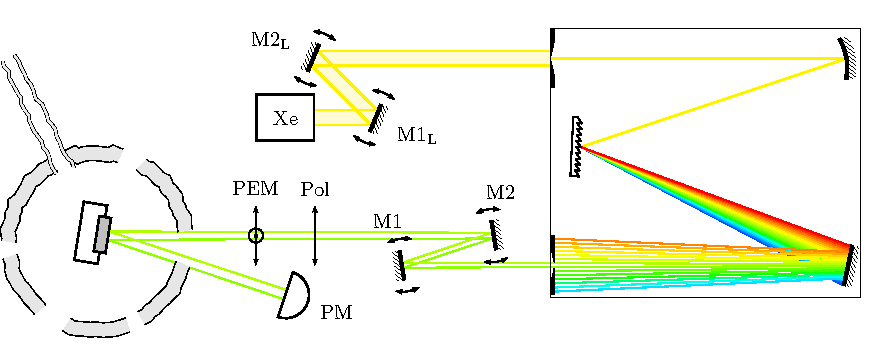
\includegraphics[width=0.8\textwidth]{figures/chap3/RAS-SETUP-gaby.pdf}
        \caption{Configuración utilizada para obtener los espectros de RDS dentro de una Cámara de Ultra Alto Vacío (UHVC)\cite{PdHGaby}.}
    \label{fig:rds-setup}
\end{figure}

El sistema utilizado para las mediciones tiene como fuente de iluminación una lampara de Xenón la cual es enfocada hacia el monocromador con el uso de un arreglo de espejos, del cual sale la luz difractada dirigida a otro arreglo de espejos los cuales dirigen la luz a la parte del sistema que controla su polarización, un prisma polarizador y un modulador fotoelástico que al pasar por ellos, obtenemos un haz de luz con una cierta polarización y que se estará modulando entre dos estados perpendiculares entre sí, incidiendo sobre la muestra para reflejarse hacia un tubo fotomultiplicador\cite{LastrasMartnez1993}.

\section{Espectroscopia Raman}
\label{sec:chap3-raman}
La Espectroscopia Raman es una técnica que se aprovecha del \textit{efecto Raman}, que describe la interaccion entre los fotones, el material que estamos estudiando y la forma en que vibra cuando la luz incide sobre una molécula, presentándose algún modo vibracional, el cual es característico de la muestra, ya que está estrechamente relacionado con la estructura molecular del material, resultando en la dispersión de fotones con diferentes frecuencias\cite{Prasankumar2016}.

\begin{figure}[h!]
    \centering
    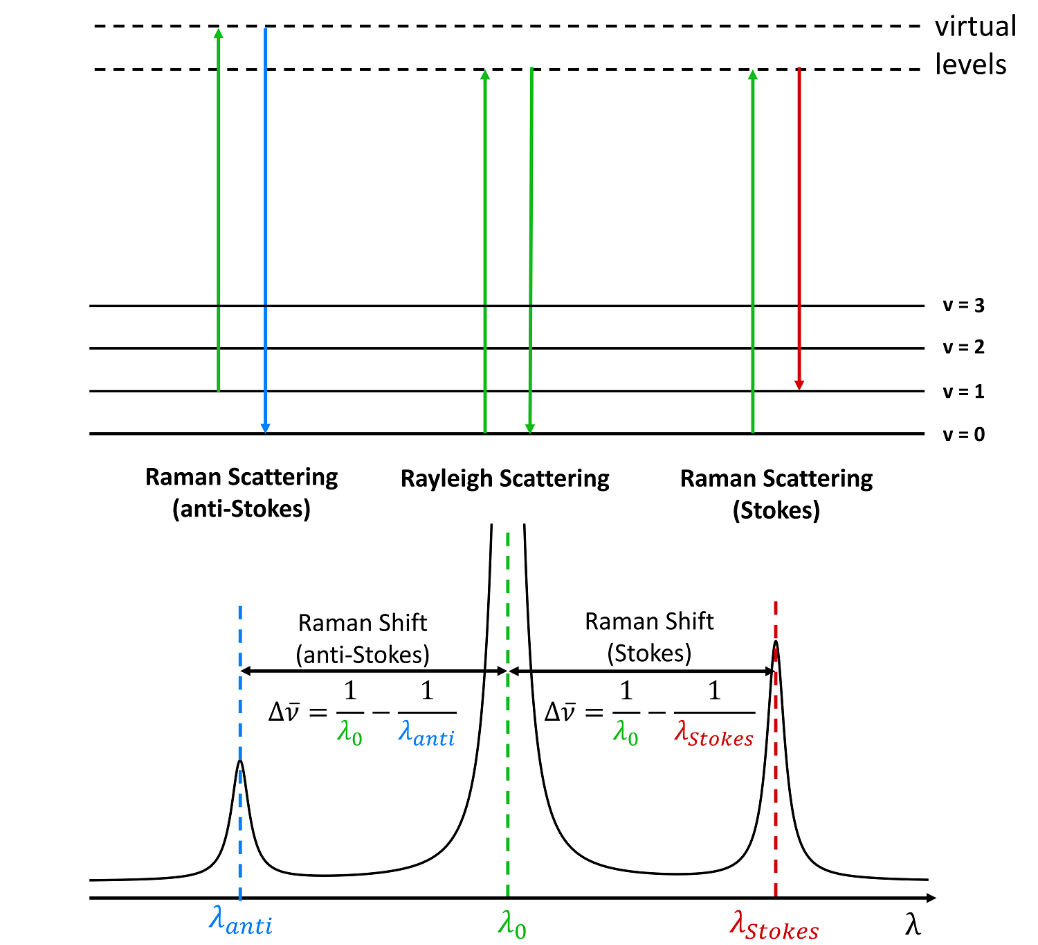
\includegraphics[width=0.8\textwidth]{figures/chap3/raman-ray-stokes-antistokes.png}
        \caption{Posibles resultados cuando un fotón choca contra la muestra, podemos observar la dependencia de energía y el tipo interacción obtenida.}
    \label{fig:raman_diagram}
\end{figure}

Cuando un fotón choca contra una molécula puede ocurrir alguno de los siguientes casos:
    \begin{itemize}
        \item Que el resultado sea un choque elástico, queriendo decir que no perderá energía por medio de efectos vibracionales, dando como resultado un fotón dispersado con la misma frecuencia. Esto se conoce como efecto Rayleigh.

        \item Que el choque resultante sea inelástico, lo que provoca que el fotón dispersado tenga una frecuencia diferente a la del incidente, teniendo el caso de una mayor frecuencia, provocando una ganancia en la energía con respecto al incidente y donde el fotón dispersado tiene menor frecuencia que el incidente, indicando que ocurrió una perdida de la energía por procesos vibracionales. Estos son nombrados efecto Anti-Stokes y efecto Stokes respectivamente.
    \end{itemize}

Por consecuencia, el efecto Stokes es utilizado para observar el \textit{efecto Raman}, siendo mas probable que este suceda porque sus fotones dispersados tienen una energía menor que su contraparte del efecto Anti-Stokes.

En el caso de los semiconductores, debido a la existencia de la red cristalina, el efecto Raman nos puede dar información sobre la cristalinidad de la muestra, debido a que cada modo vibracional tiene una frecuencia para los fotones dispersados entre estos mas se alejen o apeguen de este valor nos da una noción de que tan cristalina es la muestra\cite{Nassar2016, Qiu2021}. Otra propiedad importante es el entender el estrés al que esta sometido la muestra, por el desplazamiento de la respuesta del material en contraste con que no presente estrés\cite{Weber2000}.

En esta técnica, se utilizo el sistema comercial \textit{alpha300} de WiTec, el cual es un espectrómetro Raman acoplado a un microscopio confocal, el cual utiliza un láser de 633 nm de potencia variable, con diferentes objetivos de 10$\times$, 50$\times$ y 100$\times$.

\section{Microscopia de Fuerza Atómica}
\label{sec:chap3-afm}
La Microscopia de Fuerza Atómica (AFM), es una técnica capaz de medir la superficie de un material a nivel nanométrico utilizando como principio las fuerzas de interacción atractivas y repulsivas entre la punta del instrumento y el material. Para que la medición sea correcta, la punta debe tener una terminación en una cantidad de átomos pequeña, que al momento de experimentar una fuerza, esta provocará una deflexión en el cantiléver sobre el cual esta 
montada\cite{Binnig1986}.

La técnica de \textit{AFM}, se clasifica en tres modos de operación, que son los siguientes:
 \begin{itemize}
    \item \textit{Modo de contacto}. Con esta configuración, la punta está en \textit{contacto} con la muestra, donde la deflexión es causada por la misma morfología de la muestra, por consecuente, este modo puede causar daños sobre la superficie y se utiliza solo en contadas aplicaciones.
    
    \item \textit{Modo tapping}. En este modo, el cantiléver está oscilando a una cierta frecuencia, muy cercana a la de resonancia del mismo la cual es generada por un piezoeléctrico el cual genera vibraciones al aplicársele una corriente (\textit{piezoshaker}). El cantiléver está oscilando en frecuencia y amplitud constantes cuando no interactúa con la muestra, censando asi los cambios que ocurren en estos dos parámetros para dar información sobre la muestra\cite{Reifenberger2015-bh}.
   
    \item \textit{Modo de no contacto}. La punta se acerca tanto a la muestra, que experimenta fuerzas de atracción y repulsión hacia la misma, pero nunca hacen contacto. La deflexión del cantiléver se mide utilizando un láser y un detector sensible a la posición (plano $xz$). Una cosa importante de destacar, es que en esta configuración, obtendremos una superficie \textit{virtual}, que dependerá de la geometría de la punta, pero esto es amortiguado por medio de \textit{software}.
 \end{itemize}

 \begin{figure}[H]
    \centering
        \begin{tikzpicture}

        \begin{scope}[yshift=1cm,yscale=1]
            % wall
            \fill[pattern=north east lines] (3,0) rectangle (3.25,1);
            \draw (3.25,0) -- (3.25,1);
            % beam
            \draw[line width=1mm, gray, solid] (3.25,-1.5) [partial ellipse=90:38:4cm and 2cm];
            \draw[dashed] (3.25,0.5) -- (6.5,0.5);
            \draw[|<->|] (6.5,0.5) -- (6.5,-0.16) node[midway,right] {$L$};
            \node[ducky, rotate=-30] at (6.5,-0.47) {}; 
        \end{scope}

        \draw[fill=gray!40!black!50!white]
                {decorate[decoration={jiggly, segment length=0.25,amplitude=0.25}]
                {decorate[decoration={jiggly, segment length=1,amplitude=1}]
                {decorate[decoration={jiggly, segment length=4,amplitude=4}]     
                {(0,0) -- ++(10,0)}}}} -- ++(0,-2cm) -- ++(-10cm,0) -- cycle;
        \end{tikzpicture}
        \caption{Diagrama esquemático de la interacción entre el cantiléver y la muestra, donde se observa la deflexión \textit{L}.}
    \label{fig:afm_diagram}
\end{figure}

\section{Microscopía Óptica de Campo Cercano}
\label{sec:chap3-NSOM}

Una de las desventajas de la Microscopía Óptica es la limitante que presenta el trabajar con luz para observar los objetos, ya que la resolucion del sistema es proporcional a la longitud de onda utilizada. Cuando la muestra y la longitud de onda sean comparables en tamaño, entramos en el \textit{límite de difracción}, donde la resolución del sistema no permite distinguir los detalles del objeto observado ya que en estas condiciones la luz que usamos para iluminar es difractada.

Una de las formas para sobrepasar este limite teórico, es utilizando la Microscopía Óptica de Campo Cercano (NSOM), donde se utiliza luz para observar los objetos, pero dentro del régimen de \textit{campo cercano},